\documentclass{article}

\usepackage{amsmath}
\usepackage{graphicx}
\usepackage{subcaption}

\title{COMP9517 Assignment 1 Report}
\date{T3, 2019}
\author{Liyu Zhang Z5077914}

\begin{document}
\maketitle

\section{Introduction}
Image preprocessing involves a bunch of techniques such as image thresholding,
constrast stretching and so forth. They are widely used in digitial art to
emphasis the content and other creative fields. This assignment is focusing on
opening an image and performing a sequence of image processing operations and
produce a creative effect.

\clearpage

\section{Task 1}
\subsection{Background}
Images that composited with Red, Green and Blue colors can also be converted into gray scale image. There is this method called \textit{Weighted method or luminosity method} that the new gray scale image takes a bit from each of these three RGB channels and forms a new gray scale intensity. \\[1ex]
The task is asking us to read the input image and combine three color-bands into
one band using the following equation:

$$ I(x,y) = 0.299 * r(x,y) + 0.587 * g(x,y) + 0.114 * b(x,y) $$
\\
where $r, g \text{ and } b$ are color channels of the image $I$.

\subsection{Implementation}
This task can be done by traversing each pixel in a range of the shape ($x,y$) of image
and calculating the new value of each pixel according to the function above.
However, there is one thing to be noted that is \textbf{OpenCV} stores the color
channel values in the BGR order. Hence, we would better take that into consideration. 

\subsection{Analysis}
After applying the weighted method for each of the color channels (RGB) and combining them into one color intensity - the image is now entirely composed of one color intensity of how much dark or how much light - the image is converted into gray scale demonstrated below.

\begin{figure}[h!]
  \centering
  \begin{subfigure}[b]{0.4\linewidth}
    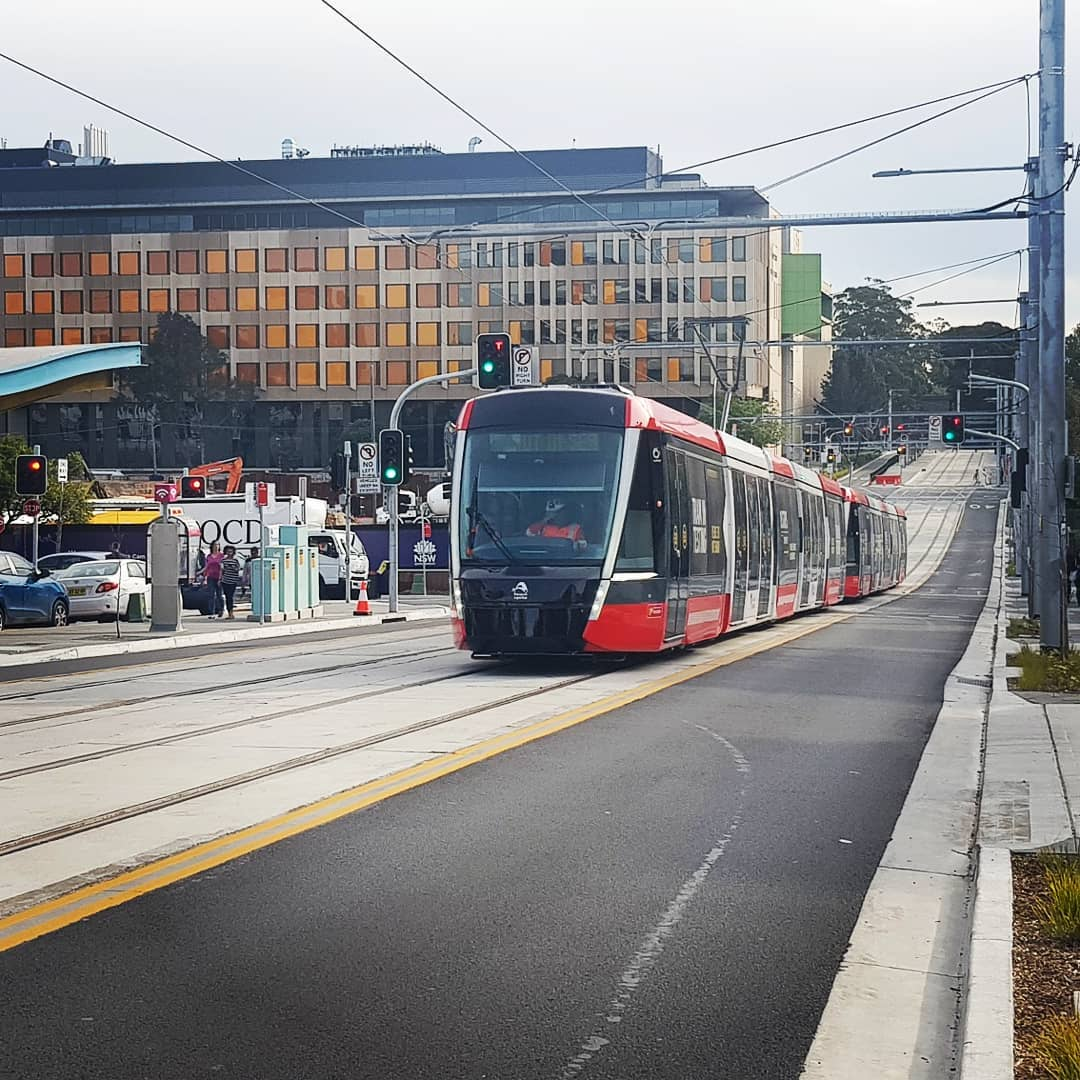
\includegraphics[width=\linewidth]{light_rail.jpg}
    \caption{Original image}
  \end{subfigure}
  \begin{subfigure}[b]{0.4\linewidth}
    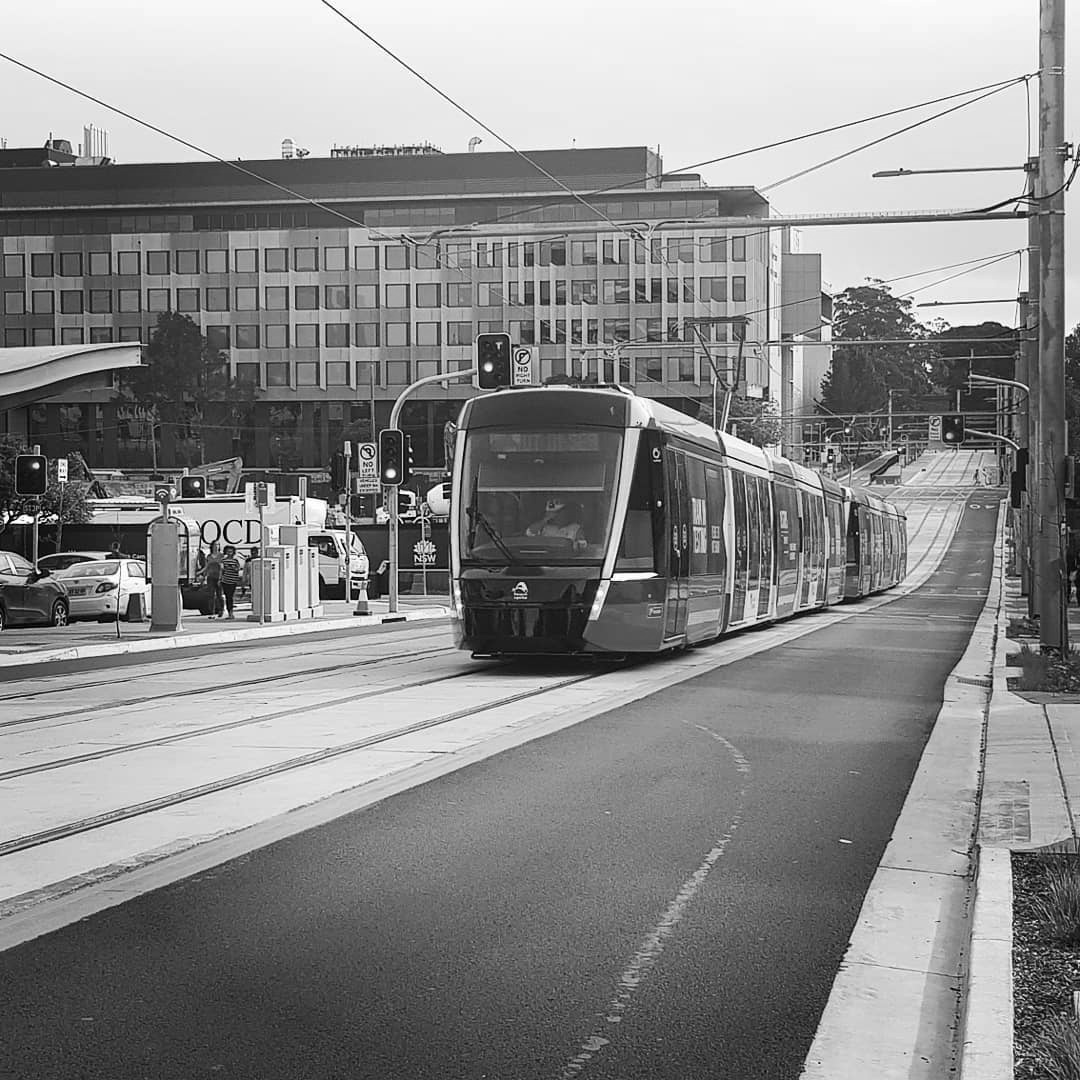
\includegraphics[width=\linewidth]{task1_light_rail_.jpg}
    \caption{Applied weighted method}
  \end{subfigure}
  \caption{Task 1 - Convert color image into gray scale image}
  \label{fig:task1}
\end{figure}

\section{Task 2}
\subsection{Background}
The task 2 is simply asking to replace each pixel in the image with the most
frequent pixel value in a range of its neighbours (also called \textit{Window}). However, as the window size has a certain affect on the sample we take into consideration, we need to test the operation with different window size (e.g., 3, 5 and 7). 

\subsection{Implementation}
The task can be achieved by traversing
each pixel and forming a window by some certain window sizes. In addition, we take the most frequent pixel value\footnote{the policy of choosing the most frequent value is arbitrarily pick the first 1 in the list} in this window. Finally, the chosen value will be assigned to the centre pixel of the window (i.e., also the pixel that composites the window), and we iterate through the whole image.

\subsection{Analysis}
With the window size increasing, some of the detail is missing by replacing the color intensity of each pixel with most frequent color intensity in its window shown below. Hence, there is no deny that the bigger of the window size is, the more detail the image loses. Therefore, the image tends to be blurry.

\begin{figure}[!h]
  \centering
  \begin{subfigure}[b]{0.4\linewidth}
    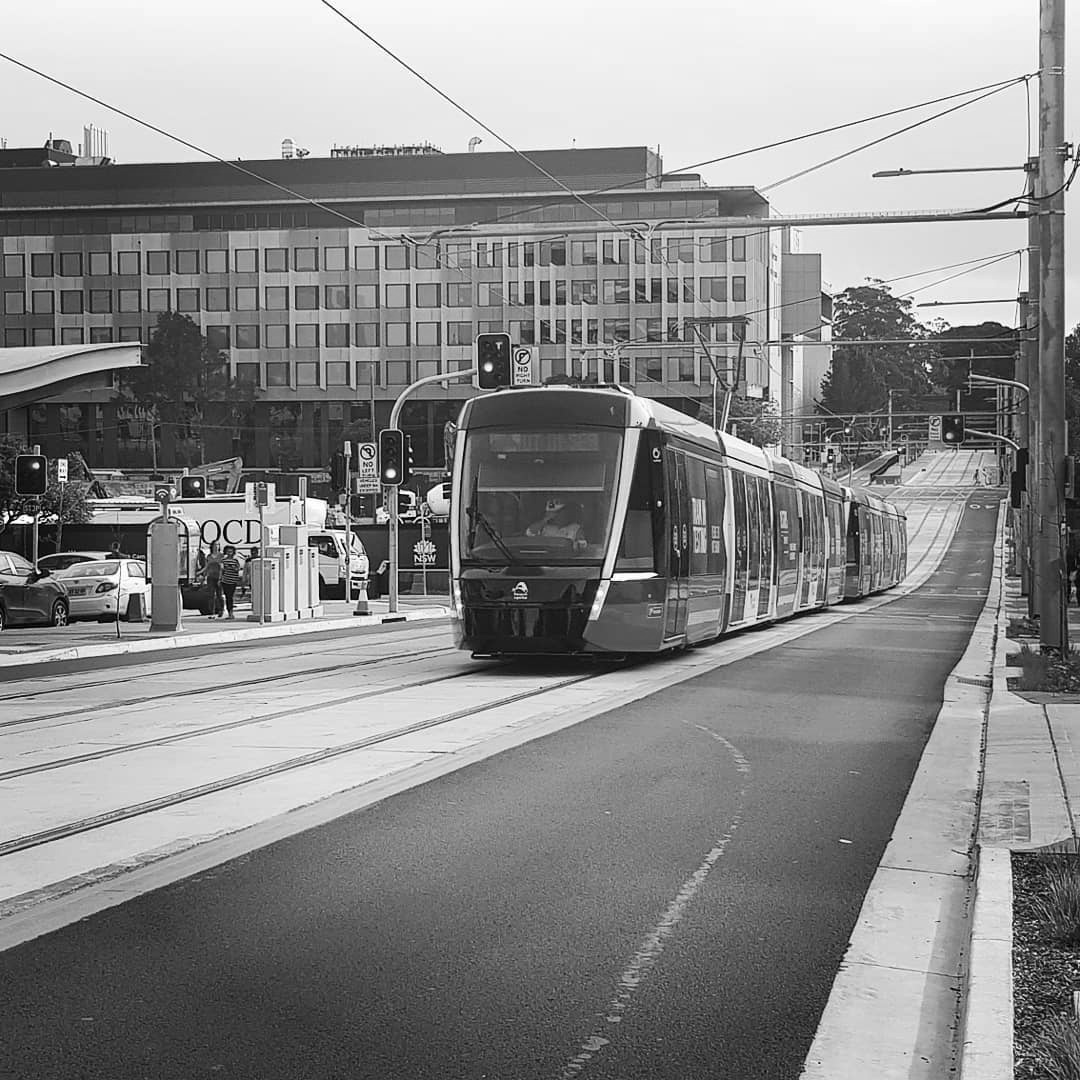
\includegraphics[width=\linewidth]{task1_light_rail_.jpg}
    \caption{Image returned by Task 1}
  \end{subfigure}
  \begin{subfigure}[b]{0.4\linewidth}
    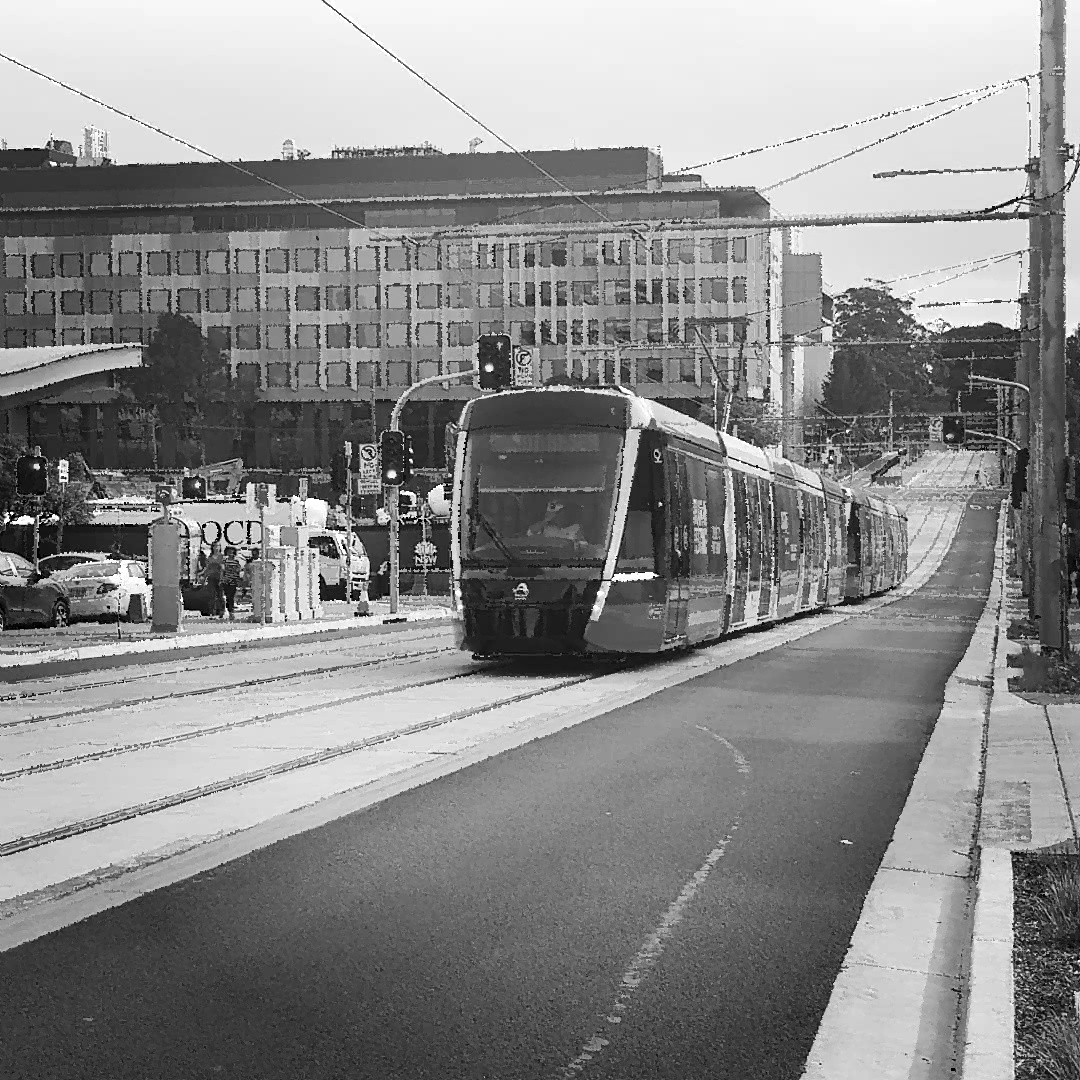
\includegraphics[width=\linewidth]{task2__light_rail_3.jpg}
    \caption{Applied window size of 3}
  \end{subfigure}
  \begin{subfigure}[b]{0.4\linewidth}
    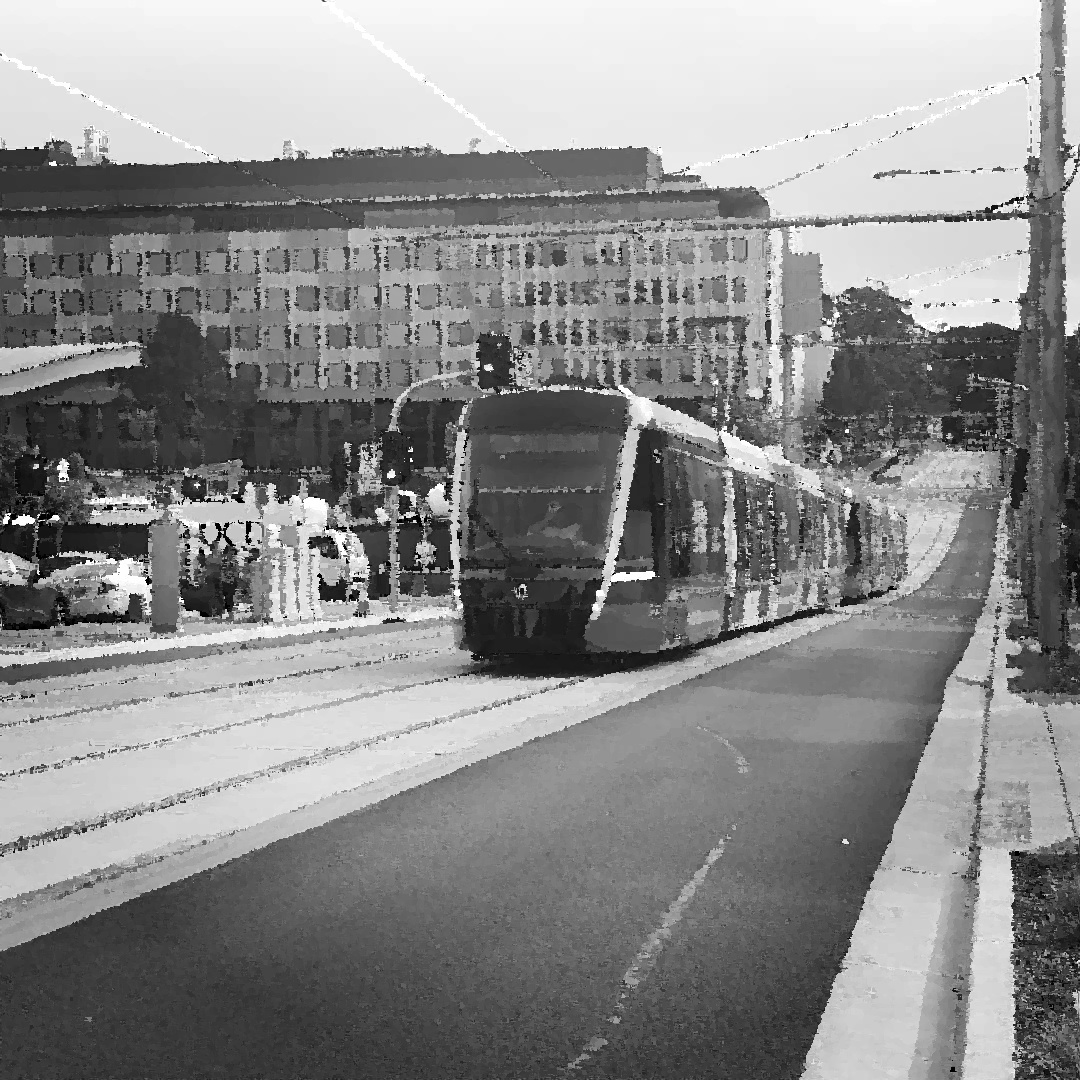
\includegraphics[width=\linewidth]{task2__light_rail_5.jpg}
    \caption{Applied window size of 5}
  \end{subfigure}
  \begin{subfigure}[b]{0.4\linewidth}
    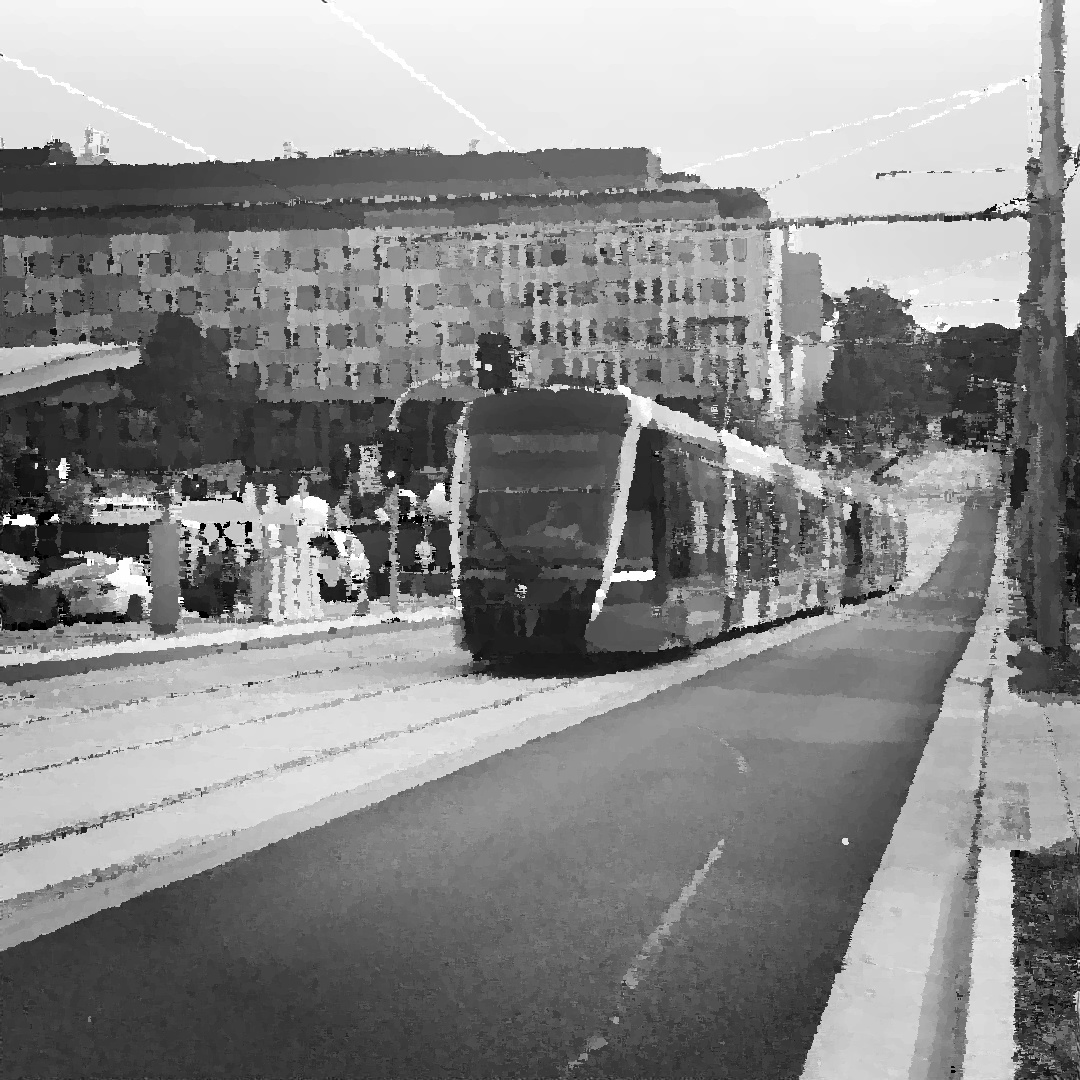
\includegraphics[width=\linewidth]{task2__light_rail_7.jpg}
    \caption{Applied window size of 7}
  \end{subfigure}
  \caption{Task 2 - Replace pixel value by the most frequent value in its window}
  \label{fig:task2}
\end{figure}

\newpage

\section{Task 3}
\subsection{Background}
Just as mentioned above in the introduction, one of the goal of image processing is to represent digital images in a more creative way. Therefore, \textit{Oil Painting Effect} cannot be neglected here.

\subsection{Implementation}
This ultimate task is asking us to achieve a visual effect called 'oil painting
effect' which can be implemented by averaging the color intensity of all pixels
that have the same pixel value in the window and replacing the original
color-bands value with it.

\subsection{Analysis}
It is shown that the bigger the window size is, the more effect we can achieve. As the window size increasing, the area where the color is similar to its neighbours. Also, the color is more blended by averaging the color of the pixel around it. Hence, we achieve an effect like Oil Painting.

\begin{figure}[!h]
  \centering
  \begin{subfigure}[b]{0.4\linewidth}
    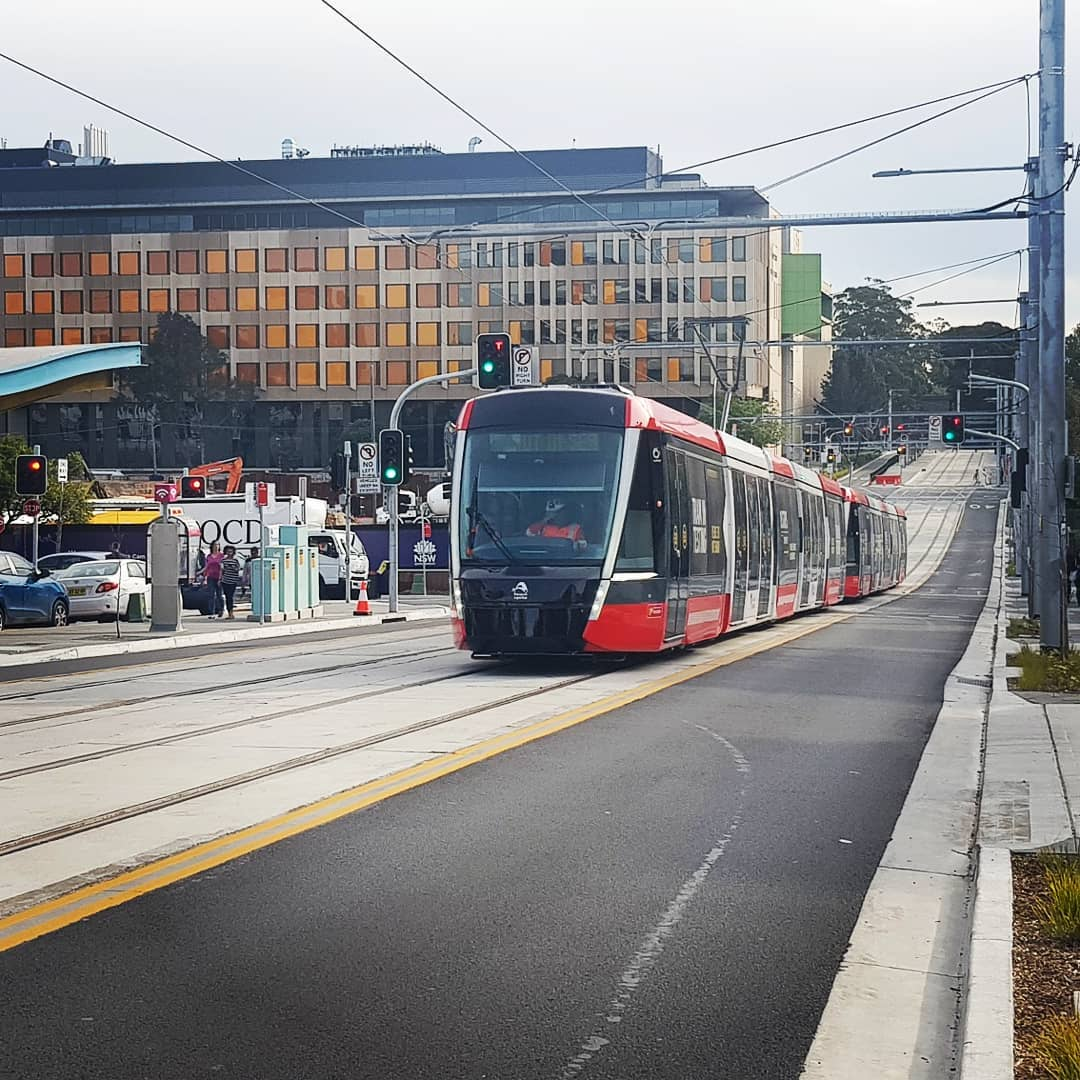
\includegraphics[width=\linewidth]{light_rail.jpg}
    \caption{Original image}
  \end{subfigure}
  \begin{subfigure}[b]{0.4\linewidth}
    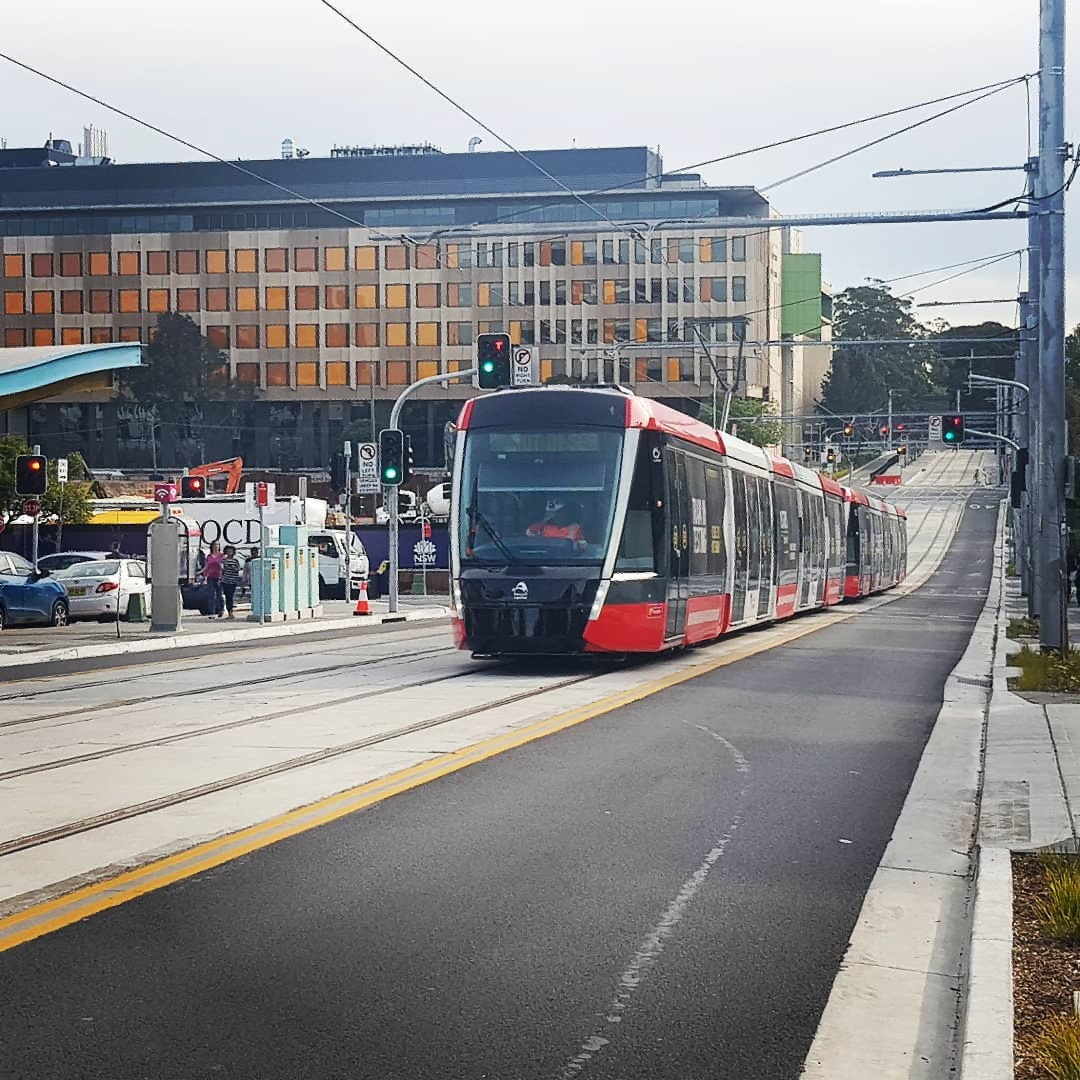
\includegraphics[width=\linewidth]{task3__light_rail_3.jpg}
    \caption{Applied window size of 3}
  \end{subfigure}
  \begin{subfigure}[b]{0.4\linewidth}
    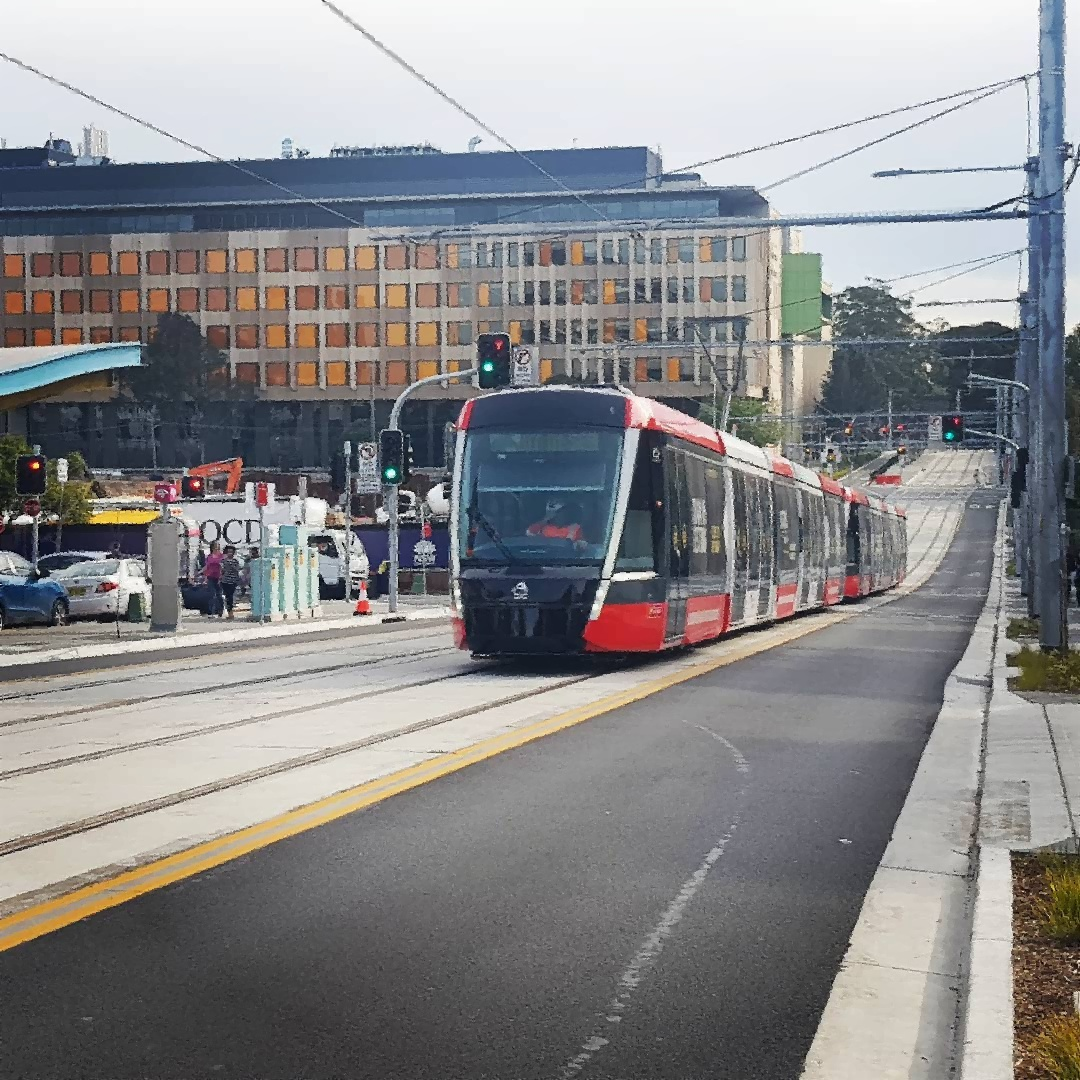
\includegraphics[width=\linewidth]{task3__light_rail_5.jpg}
    \caption{Applied window size of 5}
  \end{subfigure}
  \begin{subfigure}[b]{0.4\linewidth}
    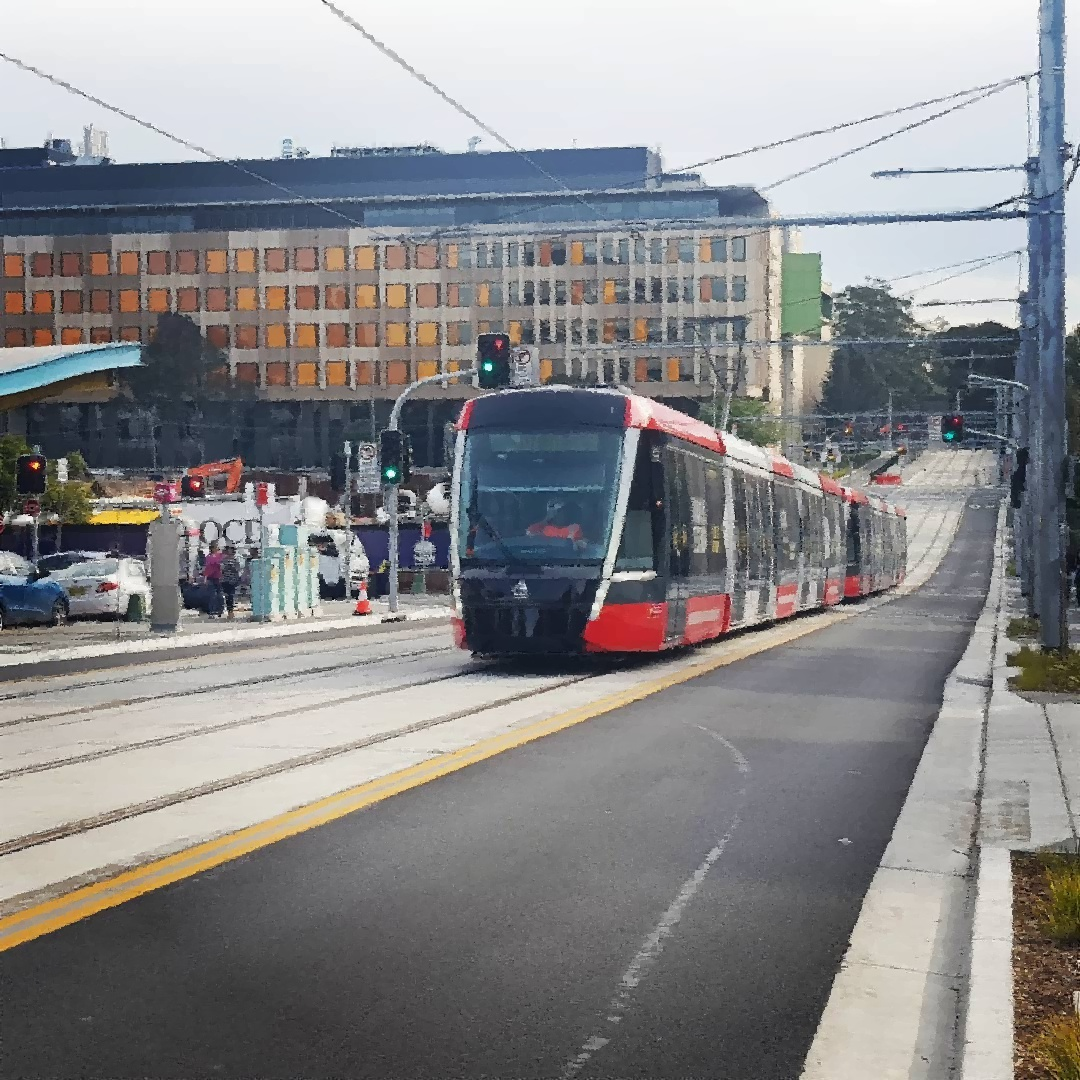
\includegraphics[width=\linewidth]{task3__light_rail_7.jpg}
    \caption{Applied window size of 7}
  \end{subfigure}
  \caption{Task 2 - Replace pixel value by the most frequent value in its window}
  \label{fig:task2}
\end{figure}

\end{document}